\documentclass[tikz,border=10pt]{standalone}
\usepackage[T1]{fontenc}
\usepackage{lmodern}
\usepackage{amsmath,amssymb}
\usepackage{tikz}
\usetikzlibrary{positioning,arrows.meta}
\begin{document}
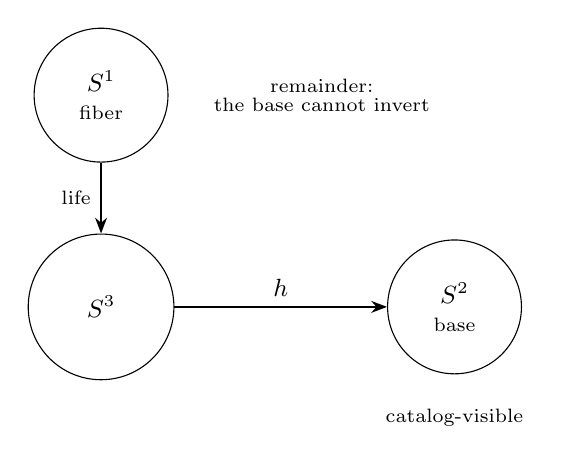
\begin{tikzpicture}[
  font=\small,
  every node/.style={align=center},
  arr/.style={-{Stealth[length=2mm]}, thick}
]
  \node[draw, circle, minimum size=1.7cm] (s1) {\(S^{1}\)\\[-1pt]\scriptsize fiber};
  \node[draw, circle, minimum size=1.85cm, below=0.9cm of s1] (s3) {\(S^{3}\)};
  \node[draw, circle, minimum size=1.7cm, right=2.7cm of s3] (s2) {\(S^{2}\)\\[-1pt]\scriptsize base};
  \draw[arr] (s1) -- node[left, font=\scriptsize] {life} (s3);
  \draw[arr] (s3) -- node[above] {\(h\)} (s2);
  \node[font=\scriptsize, below=0.32cm of s2] {catalog-visible};
  \node[font=\scriptsize, right=0.2cm of s1, xshift=0.25cm] {remainder:\\[-1pt]the base cannot invert};
\end{tikzpicture}
\end{document}
